\caulc 
%%%============= EX_1 =============%%%
\begin{ex}%[1D3H2-7]%[TDMZZ12-1-TN]%[Mui Doan]
	Giới hạn $\lim\limits_{x\to 1}\dfrac{\sqrt{x+3}-2}{|x-1|}$ bằng
	\choice
	{\True Không tồn tại}
	{$1$}
	{$0$}
	{$+\infty$}
	\loigiai{
		Ta có $\sqrt{x+3}-2=\dfrac{x+3-4}{\sqrt{x+3}+2}=\dfrac{x-1}{\sqrt{x+3}+2}$.\\
		Suy ra $\dfrac{\sqrt{x+3}-2}{|x-1|}=\dfrac{x-1}{|x-1|(\sqrt{x+3}+2)}$.\\
		Ta có
		\begin{itemize}
			\item $\lim\limits_{x\to 1^+}\dfrac{\sqrt{x+3}-2}{|x-1|}=\lim\limits_{x\to 1^+}\dfrac{x-1}{|x-1|(\sqrt{x+3}+2)}=\dfrac{1}{2+2}=\dfrac{1}{4}$.
			\item $\lim\limits_{x\to 1^-}\dfrac{\sqrt{x+3}-2}{|x-1|}=\lim\limits_{x\to 1^-}\dfrac{x-1}{-(x-1)(\sqrt{x+3}+2)}=-\dfrac{1}{2+2}=-\dfrac{1}{4}$.
		\end{itemize}
		Vì $\lim\limits_{x\to 1^+}\dfrac{\sqrt{x+3}-2}{|x-1|}\neq \lim\limits_{x\to 1^-}\dfrac{\sqrt{x+3}-2}{|x-1|}$ nên không tồn tại giới hạn $\lim\limits_{x\to 1}\dfrac{\sqrt{x+3}-2}{|x-1|}$.
	}
\end{ex}

%%%============= EX_2 =============%%%
\begin{ex}%[1D6H4-4]%[TDMZZ12]%[Nguyễn Sơn Thành]
	Nghiệm của phương trình $4^{x+1} = 2$ tương ứng là
	\choice
	{$x = \dfrac{1}{2}$}
	{$x = -1$}
	{\True $x = -\dfrac{1}{2}$}
	{$x = -\dfrac{3}{2}$}
	\loigiai{
		Ta có
		\begin{align*}
			4^{x+1} = 2
			&\Leftrightarrow \left(2^2\right)^{x+1} = 2^1\\
			&\Leftrightarrow 2^{2(x+1)} = 2^1\\
			&\Leftrightarrow 2x + 2 = 1\\
			&\Leftrightarrow 2x = -1\\
			&\Leftrightarrow x = -\dfrac{1}{2}.
		\end{align*}
		Vậy nghiệm của phương trình là $x = -\dfrac{1}{2}$.
	}
\end{ex}

%%%============= EX_3 =============%%%
\begin{ex}%[1D6H3-2]%[TDMZZ12]%[Phạm Hải Dương]
	Tập xác định của hàm số $f(x) = (x-1)^{\pi} + \sqrt{5x - 6 - x^2}$ là
	\choice
	{\True $[2;3]$}
	{$(1;+\infty)$}
	{$\mathbb{R}$}
	{$(2;3)$}
	\loigiai{
		Hàm số $f(x) = (x-1)^{\pi} + \sqrt{5x - 6 - x^2}$ xác định khi và chỉ khi
		\begin{align*}
			\heva{&x - 1 > 0 \\& -x^2 + 5x - 6 \ge 0} \Leftrightarrow \heva{&x > 1 \\ &2 \le x \le 3} \Leftrightarrow 2 \le x \le 3.
		\end{align*}
		Vậy tập xác định của hàm số là $\mathscr{D} = [2; 3]$.
	}
\end{ex}

%%%============= EX_4 =============%%%
\begin{ex}%[1D6H4-3]%[TDMZZ12]%[GVBS:Trần Phi Thoàn]
	Tập nghiệm của bất phương trình $\log(x-2) \le 1$ là
	\choice
	{$(2; 3)$}
	{$(-\infty; 12]$}
	{$(-\infty; 3]$}
	{\True $(2;12]$}
	\loigiai{
		Ta có
		\begin{align*}
			\log(x-2) \le 1\Leftrightarrow 0<x-2\le 10\Leftrightarrow 2<x\le 12.
		\end{align*}
		Vậy tập nghiệm của bất phương trình là $(2;12]$.
	}
\end{ex}

%%%============= EX_5 =============%%%
\begin{ex}%[1D7H1-2]%[TDMZZ12]%[Nguyễn Tấn Linh]
	Cho hàm số $f(x) = x^2 - 2x + 2$. Số gia của hàm số $f(x)$ tại điểm $x_0 = 2$ ứng với số gia của biến số $\Delta x = 0{,}1$ bằng
	\choice
	{$-1{,}8$}
	{$0{,}01$}
	{\True $0{,}21$}
	{$2{,}1$}
	\loigiai{
		Vì $\Delta x = 0{,}1$, $x_0 = 2 \Rightarrow x_0 + \Delta x = 2{,}1$.\\
		Thực hiện tính số gia của hàm số như sau:\\
		$\Delta y = f(x_0 + \Delta x) - f(x_0) = f(2{,}1) - f(2) = \left(2{,}1^2 - 2 \cdot 2{,}1 + 2\right) - \left(2^2 - 2 \cdot 2 + 2\right) = 0{,}21$.\\
		Vậy số gia của hàm số là $\Delta y = 0{,}21$.
	}
\end{ex}

%%%============= EX_6 =============%%%
\begin{ex}%[2D1H2-1]%[TDMZZ12]%[Bồ Văn Hậu]
	Hàm số $y=x^3-3x^2+1$ có điểm cực đại là
	\choice
	{$x=2$}
	{$y=1$}
	{\True $x=0$}
	{$y=-3$}
	\loigiai{
		Tập xác định $\mathscr{D}=\mathbb{R}$.\\
		Ta có $y'=3x^2-6x$. Cho $y'=0\Leftrightarrow 3x^2-6x=0\hoac{&x=0\\&x=2.}$\\
		Bảng biến thiên
		\begin{center}
			
\begin{tikzpicture}[scale=0.9]
				\tkzTabInit[nocadre=true,lgt=1.2,espcl=3,deltacl=0.5]
				{$x$ /0.8,$y'$ /0.8,$y$ /2}
				{$-\infty$,$0$,$2$,$+\infty$}
				\tkzTabLine{,+,0,-,0,+,}
				\tkzTabVar{-/$-\infty$,+/$1$,-/$-3$,+/$+\infty$}
			\end{tikzpicture}
		\end{center}
		Dựa vào bảng biến thiên, ta thấy hàm số đã cho có điểm cực đại là $x=0$.
	}
\end{ex}

%%%============= EX_7 =============%%%
\begin{ex}%[2D4N1-4]%[TDMZZ12]%[Võ Hiệp]
	Họ nguyên hàm của hàm số $f(x)=\mathrm{e}^{2x}-1$ là
	\choice
	{$F(x)=\mathrm{e}^{2x}-x+C$}
	{\True $F(x)=\dfrac{1}{2}\mathrm{e}^{2x}-x+C$}
	{$F(x)=\dfrac{1}{2}\mathrm{e}^{2x}-1+C$}
	{$F(x)=\dfrac{1}{2}\mathrm{e}^{2x}+x+C$}
	\loigiai{
		Ta có $\displaystyle\int\limits f(x) \mathrm{\,d}x = \displaystyle\int\limits \left(\mathrm{e}^{2x}-1 \right) \mathrm{\,d}x = \dfrac{1}{2}\mathrm{e}^{2x}-x+C$.
	}
\end{ex}

%%%============= EX_8 =============%%%
\begin{ex}%[2H5N2-3]%[TDMZZ12]%[Lê Phúc]
	Trong không gian với hệ trục tọa độ $Oxyz$, cho đường thẳng $d$ có vectơ chỉ phương là $\overrightarrow{u}=(2;1;3)$ và đi qua gốc tọa độ $O$. Phương trình tham số của đường thẳng $d$ là
	\choice
	{\True $d\colon\heva{&x=2t\\&y=t\\&z=3t}$}
	{$d\colon\heva{&x=2\\&y=1\\&z=3}$}
	{$d\colon\heva{&x=2+2t\\&y=1+t\\&z=4+3t}$}
	{$d\colon\heva{&x=1-t\\&y=2+t\\&z=3-t}$}
	\loigiai{
		Phương trình tham số của đường thẳng $d$ đi qua $O$ và có vectơ chỉ phương $\overrightarrow{u}=(2;1;3)$ là
		\begin{align*}
			d\colon\heva{&x=2t\\&y=t\\&z=3t.}
		\end{align*}
	}
\end{ex}

%%%============= EX_9 =============%%%
\begin{ex}%[2D4H2-2]%[TDMZZ12]%[Trần Văn Thiện]
	Cho $\displaystyle\int\limits_{0}^{1}2f(x)\mathrm{\,d}x=12$, $\displaystyle\int\limits_{0}^{1}3g(x)\mathrm{\,d}x=-6$. Hãy tính $\displaystyle\int\limits_{0}^{1}\left[f(x)+g(x)-2\right]\mathrm{\,d}x$.
	\choice
	{$4$}
	{\True $2$}
	{$16$}
	{$0$}
	\loigiai{
		Ta có
		\begin{itemize}
			\item $\displaystyle\int\limits_{0}^{1}2f(x)\mathrm{\,d}x=12 \Rightarrow \displaystyle\int\limits_{0}^{1}f(x)\mathrm{\,d}x=6$.
			\item $\displaystyle\int\limits_{0}^{1}3g(x)\mathrm{\,d}x=-6 \Rightarrow \displaystyle\int\limits_{0}^{1}g(x)\mathrm{\,d}x=-2$.
			\item $\displaystyle\int\limits_{0}^{1}2\mathrm{\,d}x=2$.
		\end{itemize}
		Do đó $\displaystyle\int\limits_{0}^{1}\left[f(x)+g(x)-2\right]\mathrm{\,d}x=\displaystyle\int\limits_{0}^{1}f(x)\mathrm{\,d}x+\displaystyle\int\limits_{0}^{1}g(x)\mathrm{\,d}x-\displaystyle\int\limits_{0}^{1}2\mathrm{\,d}x=6-2-2=2$.
	}
\end{ex}

%%%============= EX_10 =============%%%
\begin{ex}%[2H5N3-2]%[TDM21]%[Tên Tác Giả]
	Trong không gian hệ trục tọa độ $Oxyz$, cho mặt cầu $(S)\colon x^2 + y^2 + z^2 - 2y - 6 = 0$. Bán kính của mặt cầu $(S)$ bằng
	\choice
	{\True $\sqrt{7}$}
	{$\sqrt{6}$}
	{$3$}
	{$2\sqrt{3}$}
	\loigiai{
		Mặt cầu $(S)$ có phương trình dạng $x^2 + y^2 + z^2 - 2ax - 2by - 2cz + d = 0$ với $\heva{&a = 0 \\ &b = 1 \\ &c = 0 \\ &d = -6.}$\\
		Bán kính của mặt cầu $(S)$ là
		\begin{align*}
			R = \sqrt{a^2 + b^2 + c^2 - d} = \sqrt{0^2 + 1^2 + 0^2 - (-6)} = \sqrt{7}.
		\end{align*}
	}
\end{ex}

%%%============= EX_11 =============%%%
\begin{ex}%[2D1H5-1]%[TDMZZ12]%[Huỳnh Quốc Đạt]
	\immini{Cho hàm số $y = \dfrac{ax + b}{x + d}$ có đồ thị như hình vẽ. Dấu của các hệ số $a$, $b$, $d$ là
		\choice
		{$a > 0$, $b > 0$, $d < 0$}
		{$a < 0$, $b > 0$, $d > 0$}
		{$a > 0$, $b > 0$, $d > 0$}
		{\True $a > 0$, $b < 0$, $d < 0$}
	}{\begin{tikzpicture}[line join=round,line cap=round,>=stealth,scale=0.6]
			\tikzset{ethicknode/.style={scale=1}}
			% Vẽ hệ trục tọa độ (đỏ)
			\draw[->] (-4,0)--(5.5,0) node[below] {$x$};
			\draw[->] (0,-3)--(0,6) node[left] {$y$};
			% Vẽ các tiệm cận (đỏ,nét liền như trong hình)
			\draw (-4,1.5)--(5.5,1.5)
			(1.5,-3)--(1.5,6);
			% Vẽ đồ thị hàm số y = 1.5 - 2.25/(x-1.5) dùng scope và clip
			\begin{scope}
				\clip (-4,-3) rectangle (5.5,6);
				% Nhánh trái: đi qua (0,3)
				\draw[blue,samples=200,domain=-4:1.3,smooth,variable=\x] plot (\x,{1.5 - 2.25/(\x-1.5)});
				% Nhánh phải: đi qua (3,0)
				\draw[blue,samples=200,domain=1.7:5.5,smooth,variable=\x] plot (\x,{1.5 - 2.25/(\x-1.5)});
			\end{scope}
			\foreach \p/\ang/\lab in {
				{(0,0)}/225/O,
				{(0,3)}/180/,
				{(3,0)}/-90/
			}{
				\fill \p circle (1.5pt);
				\ifx\lab\empty \else \path \p +(\ang:12pt) node {$\lab$}; \fi
			}
		\end{tikzpicture}
	}
	\loigiai{
		Từ đồ thị ta có
		\begin{itemize}
			\item Tiệm cận đứng $x = -d$ nằm bên phải trục $Oy$ nên $-d > 0$, tức $d < 0$.
			\item Tiệm cận ngang $y = a > 0$ nằm trên trục $Ox$ nên $a>0$.
			\item Hàm cắt trục $Oy$ tại điểm có tung độ dương nên $y(0) = \dfrac{b}{d} > 0 \Rightarrow b<0$ (do $d<0$).
		\end{itemize}
		Vậy $a > 0$, $b < 0$, $d < 0$.
	}
\end{ex}

%%%============= EX_12 =============%%%
\begin{ex}%[2D3H1-2]%[TDM31]%[Tên Tác Giả]
	Cho mẫu số liệu ghép nhóm $M$ có tất cả $6$ nhóm với độ dài bằng nhau. Biết rằng phần tử đại diện của nhóm thứ $4$ hơn đầu mút trái của nhóm thứ $2$ là $6$ đơn vị. Hãy xác định khoảng biến thiên của mẫu số liệu $M$?
	\choice
	{\True $14{,}4$}
	{$18$}
	{$12$}
	{$24{,}6$}
	\loigiai{
		Giả sử mẫu số liệu ghép nhóm $M$ gồm $6$ nhóm có dạng $[a_1; a_2), [a_2; a_3), \dots, [a_6; a_7]$.\\
		Gọi $c$ là độ dài của mỗi nhóm ($c > 0$). Khi đó $a_{i+1} - a_i = c$ với mọi $i \in \{1; 2; \dots; 6\}$.\\
		Đầu mút trái của nhóm thứ $2$ là $a_2 = a_1 + c$.\\
		Nhóm thứ $4$ là $[a_4; a_5) = [a_1 + 3c; a_1 + 4c)$.\\
		Phần tử đại diện của nhóm thứ $4$ là
		\begin{align*}
			x_4 = \dfrac{a_4 + a_5}{2} = \dfrac{(a_1 + 3c) + (a_1 + 4c)}{2} = a_1 + 3{,}5c.
		\end{align*}
		Theo giả thiết, phần tử đại diện của nhóm thứ $4$ hơn đầu mút trái của nhóm thứ $2$ là $6$ đơn vị nên ta có phương trình:
		\begin{align*}
			x_4 - a_2 = 6 \Leftrightarrow (a_1 + 3{,}5c) - (a_1 + c) = 6 \Leftrightarrow 2{,}5c = 6 \Leftrightarrow c = 2{,}4.
		\end{align*}
		Khoảng biến thiên của mẫu số liệu ghép nhóm $M$ là
		\begin{align*}
			R = a_7 - a_1 = 6c = 6 \cdot 2{,}4 = 14{,}4.
		\end{align*}
	}
\end{ex}
\cauds
%%%============= EX_13 =============%%%
\begin{ex}%[2H5H1-5]%[TDMZZ12]%[Dương Công Tạo]
	Trong không gian $Oxyz$, cho điểm $A(1;0;5)$, $B(-1;2;1)$, $C(3;4;3)$.
	\choiceTF
	{\True $\overrightarrow{AB} = (-2;2;-4)$, $\overrightarrow{AC} = (2;4;-2)$}
	{\True Phương trình tổng quát của mặt phẳng $(ABC)$ là $x-y-z+4=0$}
	{\True Tập hợp các điểm cách đều $A$ và $B$ là mặt phẳng có phương trình tổng quát là \break$x - y + 2z - 5 = 0$}
	{\True Nếu $I(a;b;c)$ là tâm đường tròn ngoại tiếp của $\triangle ABC$ thì $a+b+c=6$}
	\loigiai{
		\begin{itemchoice}
			\itemch Ta có $\overrightarrow{AB} = (-2;2;-4)$, $\overrightarrow{AC} = (2;4;-2)$.
			\itemch Ta có $\left[\overrightarrow{AB},\overrightarrow{AC}\right]=(12;-12;-12)$.\\
			Chọn một vectơ pháp tuyến của mặt phẳng $(ABC)$ là $\overrightarrow{n}=(1;-1;-1)$ thì mặt phẳng $(ABC)$ có phương trình là \[1\cdot(x-1)-1\cdot(y-0)-1\cdot(z-5)=0\text{ hay }x-y-z+4=0.\]
			\itemch Gọi $M(x;y;z)$ là các điểm cách đều hai điểm $A$ và $B$.\\
			Ta có \allowdisplaybreaks
			\begin{align*}
				AM^2=BM^2&\Leftrightarrow (x-1)^2+y^2+(z-5)^2=(x+1)^2+(y-2)^2+(z-1)^2\\
				&\Leftrightarrow 4x-4y+8z-20=0\\
				&\Leftrightarrow x-y+2z-5=0.
			\end{align*}
			\itemch Ta có
			\begin{itemize}
				\item $\overrightarrow{AB} = (-2;2;-4) \Rightarrow AB=\sqrt{24}$.
				\item $\overrightarrow{AC} = (2;4;-2) \Rightarrow AC=\sqrt{24}$.
				\item $\overrightarrow{BC} = (4;2;2) \Rightarrow BC=\sqrt{24}$.
			\end{itemize}
			Suy ra $\triangle ABC$ đều. Khi đó, tâm đường tròn ngoại tiếp $\triangle ABC$ cũng chính là trọng tâm $G$.\\
			Do đó $G(1;2;3)$. Vậy $a+b+c=1+2+3=6$.
		\end{itemchoice}
	}
\end{ex}

%%%============= EX_14 =============%%%
\begin{ex}%[2D4V3-4]%[TDMZZ12]%[Văn Minh Thoại]
	\immini[thm]{
		Một biển quảng cáo hình chữ nhật $ABCD$ có kích thước $AB=180$ cm, $AD=240$ cm. Phần được tô mờ (phần ở giữa) sẽ được dùng để in nội dung quảng cáo như hình vẽ. Tiến hành gắn hệ trục toạ $Oxy$ vào biển quảng cáo (đơn vị dài trên mỗi trục là $1$ cm) sao cho gốc toạ độ $O$ nằm trong hình chữ nhật, cách cạnh $AB$ là $100$ cm, cách cạnh $BC$ là $120$ cm. Ta dùng đồ thị $(C)$ của hàm số $y=\dfrac{a}{x}$, sao cho nó đi qua trung điểm của cạnh $BC$, dựa vào đồ thị $(C)$ này ta tô đậm được phần cần in quảng cáo
	}{
		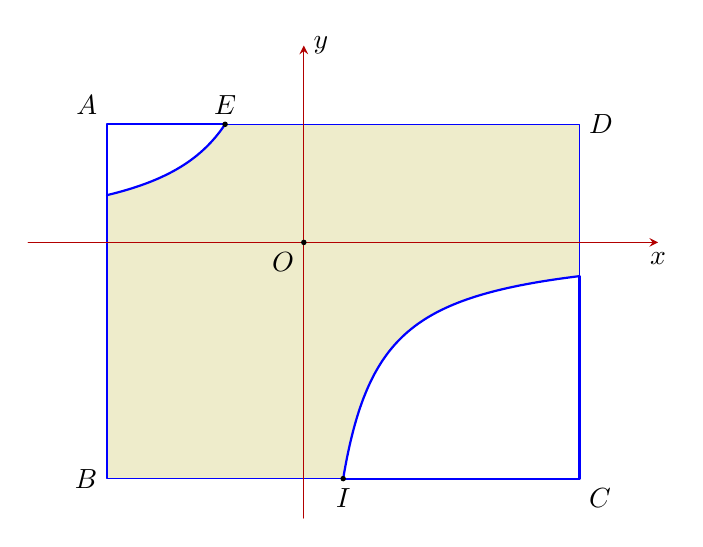
\begin{tikzpicture}[>=stealth,line join=round,line cap=round,every node/.style={font=\normalsize},declare function={a = -1.5; xmin = -3.5; xmax = 4.5; ymin = -3.5; ymax = 2.5; }]
			\path
			(-2.5,1.5) coordinate (A)
			(-2.5,-3) coordinate (B)
			(3.5,-3) coordinate (C)
			(3.5,1.5) coordinate (D)
			(-1,1.5) coordinate (E)
			(0.5,-3) coordinate (I)
			(0,0) coordinate (O);
			\pgfmathsetmacro{\giaoDC}{-3/7}
			\fill[olive!15]
			(B) -- (-2.5,{a/(-2.5)})
			-- plot[domain=-2.5:-1,smooth,samples=150] (\x,{a/\x})
			-- (D) -- (3.5,{a/3.5})
			-- plot[domain=3.5:0.5,smooth,samples=150] (\x,{a/\x})
			-- cycle;
			\draw[blue] (B) rectangle (D);
			\draw[thick,blue,smooth,samples=150,domain=-2.5:-1]
			plot (\x,{a/\x});
			\draw[thick,blue,smooth,samples=150,domain=0.5:3.5]
			plot (\x,{a/\x});
			\draw[thick,blue](I)--(C)--(3.5,\giaoDC)
			(-2.5,0.6)--(A)--(E);
			\draw[->,red!70!black] (xmin,0) -- (xmax,0) node[below,text=black] {$x$};
			\draw[->,red!70!black] (0,ymin) -- (0,ymax) node[right,text=black] {$y$};
			\fill (O) circle (1pt) node[below left] {$O$};
			\fill (E) circle (1pt) node[above] {$E$};
			\fill (I) circle (1pt) node[below] {$I$};
			\node[above left] at (A) {$A$};
			\node[left] at (B) {$B$};
			\node[below right] at (C) {$C$};
			\node[right] at (D) {$D$};
		\end{tikzpicture}
	}
	\choiceTF
	{Toạ độ của điểm $E$ là $E(20;100)$}
	{\True Phương trình $AD$, $BC$ lần lượt là $AD\colon y=60$, $BC\colon y=-120$}
	{$a=-2\,000$}
	{Diện tích cần in nội dung quảng cáo bằng $3{,}09$ \textit{(đơn vị tính theo mét vuông và làm tròn kết quả đến hàng phần trăm)}}
	\loigiai{
		Chọn hệ trục tọa độ $Oxy$ như hình vẽ, với gốc tọa độ $O(0;0)$.\\
		Theo giả thiết, gốc $O$ cách cạnh $AB$ là $100$ cm và cạnh $AB$ nằm bên trái trục $Oy$ nên phương trình đường thẳng chứa cạnh $AB$ là $x=-100$.\\
		Do $AD=240$ cm nên phương trình đường thẳng chứa cạnh $CD$ là $x=-100+240=140$.\\
		Gốc $O$ cách cạnh $BC$ là $120$ cm và cạnh $BC$ nằm bên dưới trục $Ox$ nên phương trình đường thẳng chứa cạnh $BC$ là $y=-120$.\\
		Do $AB=180$ cm nên phương trình đường thẳng chứa cạnh $AD$ là $y=-120+180=60$.\\
		Từ đó, tọa độ các đỉnh của hình chữ nhật $ABCD$ là $A(-100;60)$, $B(-100;-120)$, $C(140;-120)$ và $D(140;60)$.\\
		Gọi $I$ là trung điểm của cạnh $BC$. Hoành độ của $I$ là $x_I=\dfrac{-100+140}{2}=20\Rightarrow I(20;-120)$.\\
		Vì đồ thị $(C)$ của hàm số $y=\dfrac{a}{x}$ đi qua trung điểm $I$ của $BC$ nên
		\[-120 = \dfrac{a}{20} \Leftrightarrow a = -2\,400.\]
		\begin{itemchoice}
			\itemch Điểm $E$ là giao điểm của nhánh đồ thị $(C)$ (với $x<0$) và cạnh $AD$ (có phương trình $y=60$).\\
			Ta có $60=-\dfrac{2\,400}{x}\Leftrightarrow x=-40$. Suy ra $E(-40; 60)$.
			\itemch Phương trình $AD\colon y=60$, $BC\colon y=-120$.
			\itemch Theo kết quả tính ở trên, $a=-2\,400$.
			\itemch
			\begin{center}
				\begin{tikzpicture}[>=stealth,line join=round,line cap=round,every node/.style={font=\footnotesize},declare function={a = -1.5; xmin = -3.5; xmax = 4.5; ymin = -3.5; ymax = 2.5; }]
					\path
					(-2.5,1.5) coordinate (A)
					(-2.5,-3) coordinate (B)
					(3.5,-3) coordinate (C)
					(3.5,1.5) coordinate (D)
					(-1,1.5) coordinate (E)
					(0.5,-3) coordinate (I)
					(0,0) coordinate (O);
					\pgfmathsetmacro{\giaoDC}{-3/7}
					\fill[pattern = north east lines,pattern color = red] (E)--++(0,-4.5)--(B)--(-2.5,0.6)--plot[smooth,samples=150,domain=-2.5:-1]
					(\x,{a/\x})--cycle;
					\fill[pattern = dots,pattern color = green] (E)--++(0,-4.5)--(B)--(I)--++(0,4.5)--cycle;
					\fill[pattern = north east lines,pattern color = magenta] (I)--++(0,4.5)--(D)--(3.5,\giaoDC)--plot[thick,blue,smooth,samples=150,domain=3.5:0.5]
					(\x,{a/\x})--cycle;
					\draw[blue] (B) rectangle (D);
					\draw[thick,blue,smooth,samples=150,domain=-2.5:-1]
					plot (\x,{a/\x});
					\draw[thick,blue,smooth,samples=150,domain=0.5:3.5]
					plot (\x,{a/\x});
					\draw[thick,blue](I)--(C)--(3.5,\giaoDC)
					(-2.5,0.6)--(A)--(E);
					\draw[->,red!70!black] (xmin,0) -- (xmax,0) node[below,text=black] {$x$};
					\draw[->,red!70!black] (0,ymin) -- (0,ymax) node[right,text=black] {$y$};
					\fill (O) circle (1pt) node[below left] {$O$};
					\fill (E) circle (1pt) node[above] {$E$};
					\fill (I) circle (1pt) node[below] {$I$};
					\node[above left] at (A) {$A$};
					\node[left] at (B) {$B$};
					\node[below right] at (C) {$C$};
					\node[right] at (D) {$D$};
					\fill[ball color=black] (-2.5,0) circle (1pt) node[shift=(-145:0.6)] {$-100$};
					\fill[ball color=black] (-1,0) circle (1pt) node[shift=(-90:0.4)] {$-40$};
					\fill[ball color=black] (0.5,0) circle (1pt) node[shift=(-90:0.4)] {$20$};
					\fill[ball color=black] (3.5,0) circle (1pt) node[shift=(45:0.6)] {$140$};
				\end{tikzpicture}
			\end{center}
			Diện tích phần tô đậm $S$ được tính bằng tổng diện tích của $3$ miền phẳng giới hạn bởi đồ thị $(C)$ và các cạnh của hình chữ nhật là
			\allowdisplaybreaks
			\begin{align*}
				S &= \displaystyle\int\limits_{-100}^{-40} \left( -\dfrac{2\,400}{x} - (-120) \right) \mathrm{\,d}x + \displaystyle\int\limits_{-40}^{20} \big(60 - (-120)\big) \mathrm{\,d}x + \displaystyle\int\limits_{20}^{140} \left(60 - \left( -\dfrac{2\,400}{x} \right) \right) \mathrm{\,d}x \\
				&= \left(-2\,400\ln|x| + 120x \right)\Bigg|_{-100}^{-40} + 180x\Bigg|_{-40}^{20} + \left(60x + 2\,400\ln|x| \right)\Bigg|_{20}^{140} \\
				&= \left(7\,200 + 2\,400\ln\dfrac{5}{2} \right) + 10\,800 + \left(7\,200 + 2\,400\ln 7 \right) \\
				&= 25\,200 + 2\,400\ln\dfrac{35}{2} \text{ (cm}^2) = 2{,}52 + 0{,}24\ln\dfrac{35}{2} \text{ (m}^2) \approx 3{,}21 \text{ (m}^2).
			\end{align*}
			Diện tích cần in là khoảng $3{,}21$ m$^2$.
		\end{itemchoice}
	}
\end{ex}

%%%============= EX_15 =============%%%
\begin{ex}%[2D6V2-3]%[TDMZZ12]%[Vũ Hồng Toàn]
	Một công ty có giao cho ba xí nghiệp sản xuất $10\,000$ sản phẩm một loại mặt hàng. Xí nghiệp I sản xuất $5\,000$ sản phẩm với tỉ lệ phế phẩm là $3\%$, xí nghiệp II sản xuất $3\,000$ sản phẩm với tỉ lệ phế phẩm là $4\%$, xí nghiệp III có tỉ lệ phế phẩm là $5\%$. Chọn ngẫu nhiên một sản phẩm của loại mặt hàng này.
	\choiceTF
	{Xác suất chọn được phế phẩm, nếu biết sản phẩm đó của xí nghiệp II, là $0{,}03$}
	{\True Tỉ lệ để chọn được phế phẩm là $3{,}7\%$}
	{Biết đã chọn được phế phẩm, xác suất nó là do xí nghiệp II sản xuất là $\dfrac{3}{16}$}
	{Biết chọn được sản phẩm không phải của xí nghiệp I, xác suất chọn được phế phẩm là $4{,}52\%$ (theo đơn vị phần trăm và làm tròn kết quả đến hàng phần trăm)}
	\loigiai{
		Gọi $A_1$, $A_2$, $A_3$ lần lượt là biến cố sản phẩm chọn ra thuộc xí nghiệp I, II, III.\\
		Ta có $\mathrm{P}\left(A_1\right) = \dfrac{5\,000}{10\,000} = 0{,}5$; $\mathrm{P}\left(A_2\right) = \dfrac{3\,000}{10\,000} = 0{,}3$; $\mathrm{P}\left(A_3\right) = \dfrac{10\,000 - 5\,000 - 3\,000}{10\,000} = 0{,}2$.\\
		Gọi $B$ là biến cố sản phẩm chọn ra là phế phẩm.\\
		Theo đề bài $\mathrm{P}\left(B\mid A_1\right) = 3\% = 0{,}03$; $\mathrm{P}\left(B\mid A_2\right) = 4\% = 0{,}04$; $\mathrm{P}\left(B\mid A_3\right) = 5\% = 0{,}05$.\\
		Ta có sơ đồ hình cây như sau
		\begin{center}
			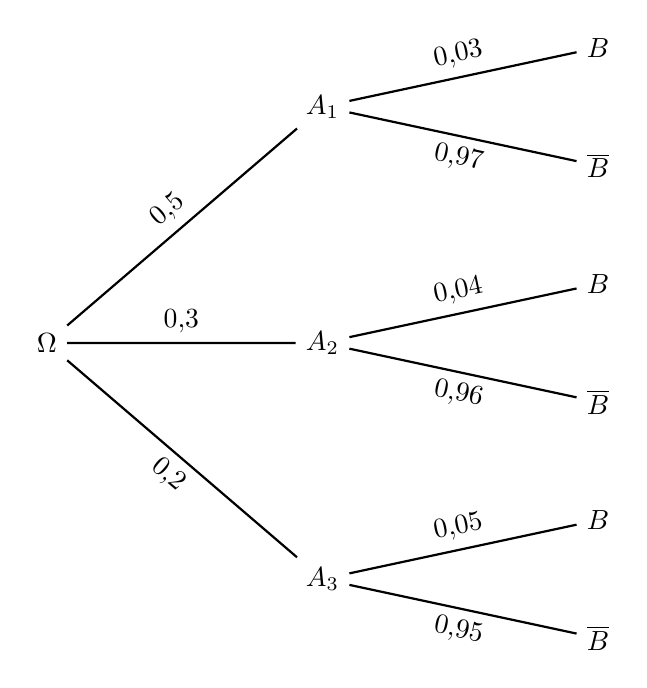
\begin{tikzpicture}[grow=right, sloped, level distance=3.5cm, 
				level 1/.style={sibling distance=3cm}, 
				level 2/.style={sibling distance=1.5cm},
				thick, >=stealth]
				\node {$\Omega$}
				child {node {$A_3$}
					child {node {$\overline{B}$} edge from parent node[below] {$0{,}95$}}
					child {node {$B$} edge from parent node[above] {$0{,}05$}}
					edge from parent node[below] {$0{,}2$}
				}
				child {node {$A_2$}
					child {node {$\overline{B}$} edge from parent node[below] {$0{,}96$}}
					child {node {$B$} edge from parent node[above] {$0{,}04$}}
					edge from parent node[above] {$0{,}3$}
				}
				child {node {$A_1$}
					child {node {$\overline{B}$} edge from parent node[below] {$0{,}97$}}
					child {node {$B$} edge from parent node[above] {$0{,}03$}}
					edge from parent node[above] {$0{,}5$}
				};
			\end{tikzpicture}
		\end{center}
		\begin{itemchoice}
			\itemch Xác suất chọn được phế phẩm nếu biết sản phẩm đó của xí nghiệp II là \[\mathrm{P}\left(B\mid A_2\right) = 0{,}04.\]
			\itemch Tỉ lệ chọn được phế phẩm là xác suất đầy đủ.
			\begin{align*}
				\mathrm{P}\left(B\right) &= \mathrm{P}\left(A_1\right) \cdot \mathrm{P}\left(B\mid A_1\right) + \mathrm{P}\left(A_2\right) \cdot \mathrm{P}\left(B\mid A_2\right) + \mathrm{P}\left(A_3\right) \cdot \mathrm{P}\left(B\mid A_3\right)\\& = 0{,}5 \cdot 0{,}03 + 0{,}3 \cdot 0{,}04 + 0{,}2 \cdot 0{,}05\\& = 0{,}037 = 3{,}7\%.
			\end{align*}
			\itemch Xác suất phế phẩm đó do xí nghiệp II sản xuất là
			\begin{align*}
				\mathrm{P}\left(A_2\mid B\right) = \dfrac{\mathrm{P}\left(A_2\right) \cdot \mathrm{P}\left(B\mid A_2\right)}{\mathrm{P}\left(B\right)} = \dfrac{0{,}3 \cdot 0{,}04}{0{,}037} = \dfrac{12}{37}.
			\end{align*}
			\itemch Xác suất chọn được phế phẩm trong trường hợp này là
			\begin{align*}
				\mathrm{P}\left(B\mid A_2 \cup A_3\right) = \dfrac{\mathrm{P}\left(B \cap A_2\right) + \mathrm{P}\left(B \cap A_3\right)}{\mathrm{P}\left(A_2\right) + \mathrm{P}\left(A_3\right)} = \dfrac{0{,}3 \cdot 0{,}04 + 0{,}2 \cdot 0{,}05}{0{,}3 + 0{,}2} = 0{,}044 = 4{,}4\%.
			\end{align*}
		\end{itemchoice}
	}
\end{ex}

%%%============= EX_16 =============%%%
\begin{ex} %[2D4V1-6]%[TDMZZ12]%[Hà Văn Hảo]
	Một hội trường có tất cả $N_0 = 300$ người bắt đầu cùng tranh luận một vấn đề. Ở thời điểm ban đầu số người ủng hộ là $30$ và còn lại là phản đối. Biết rằng tốc độ tăng số lượng người ủng hộ tỉ lệ thuận với số lượng người phản đối: $N'(t) = k M(t)$, với $k$ là số thực dương, thời gian $t$ ($t \ge 0$) tính theo giờ, $N'(t)$ là tốc độ tăng số người ủng hộ (người/giờ), $M(t)$ là số lượng người phản đối sau $t$ giờ. Sau $1$ giờ số lượng người phản đối còn lại $220$ người.
	\choiceTF
	{$M(0) = 300$ người}
	{\True $N(1) = 80$ người}
	{$k = \dfrac{27}{22}$}
	{\True Sau $3$ giờ thì tổng số người ủng hộ là $154$ người \textit{(làm tròn kết quả đến hàng đơn vị)}}
	\loigiai{
		Gọi $N(t)$ là số người ủng hộ và $M(t)$ là số người phản đối tại thời điểm $t$.\\
		Tổng số người không đổi nên $N(t) + M(t) = 300 \Rightarrow M(t) = 300 - N(t)$.
		\begin{itemchoice}
			\itemch Tại thời điểm $t=0$, số người ủng hộ là $N(0) = 30$. \\
			Do đó số người phản đối là $M(0) = 300 - 30 = 270$ người.
			\itemch Sau $1$ giờ, số người phản đối là $M(1) = 220$ người.\\
			Suy ra số người ủng hộ là $N(1) = 300 - 220 = 80$ người.
			\itemch Ta có phương trình vi phân $N'(t) = k[300 - N(t)]$.\\
			Đặt $u(t) = 300 - N(t) \Rightarrow u'(t) = -N'(t)$.\\
			Khi đó $-u'(t) = k \cdot u(t) \Rightarrow \dfrac{u'(t)}{u(t)} = -k$.\\
			Lấy nguyên hàm hai vế $\ln|u(t)| = -kt + C \Rightarrow u(t) = \mathrm{e}^{-kt+C} = \mathrm{e}^C \cdot \mathrm{e}^{-kt}$.\\
			Tại $t=0$, $u(0) = 300 - N(0) = 270 \Rightarrow \mathrm{e}^C = 270$.\\
			Suy ra $M(t) = 270 \cdot \mathrm{e}^{-kt}$ và $N(t) = 300 - 270 \cdot \mathrm{e}^{-kt}$.\\
			Tại $t=1$, $M(1) = 270 \cdot \mathrm{e}^{-k} = 220 \Rightarrow \mathrm{e}^{-k} = \dfrac{22}{27} \Rightarrow k = -\ln\left(\dfrac{22}{27}\right) = \ln\left(\dfrac{27}{22}\right)$. 
			\itemch Tại thời điểm $t=3$, số người ủng hộ là
			$N(3) = 300 - 270 \cdot \mathrm{e}^{-3k} = 300 - 270 \cdot (\mathrm{e}^{-k})^3$.\\
			Thay $\mathrm{e}^{-k} = \dfrac{22}{27}$ vào ta được
			\[N(3) = 300 - 270 \cdot \left(\dfrac{22}{27}\right)^3 = 300 - \dfrac{106\,480}{729} = \dfrac{112\,220}{729} \approx 154.\]
			Vậy sau $3$ giờ thì tổng số người ủng hộ là $154$ người.
		\end{itemchoice}
	}
\end{ex}
\caukq
%%%============= EX_17 =============%%%
\begin{ex}%[0D3V2-6]%[TDMZZ12]%[Duong Xuan Loi]
	Bác Bình chỉ có $40$ mét chiều dài hàng rào để quây thành hai ô để chăn nuôi ở bờ sông. Người này thiết kế hình dạng hàng rào như hình vẽ gồm một đoạn song song với bờ sông, ba đoạn bằng nhau song song với nhau và vuông góc với bờ sông. Hãy tính theo mét vuông, tổng diện tích lớn nhất mà bác Bình quây được (làm tròn kết quả đến hàng đơn vị)?
	\begin{center}
		\begin{tikzpicture}[scale=0.8, font=\footnotesize, line join=round, line cap=round, >=stealth]
			\fill[white!80!green] (-1,-.5) rectangle (12.5,2);
			\fill[white!70!cyan] (-1,2) rectangle (12.5,3);
			\fill[white!90!brown] (0,0)--(10,0)--(11.8,2)--(1.8,2)--cycle;
			
			\tikzset{tru/.pic=
				{\shade[top color=brown, bottom color=brown!50, shading angle={100}, fill=brown!70,rounded corners=0.5ex,thick]
					(0:0)--++(90:.8)--++(60:.2)--++(-60:.2)--++(-90:.8)--cycle;
					\draw[fill=black!50] (.1,.6) circle (.2mm);	}
			}
			\draw[line width=1mm,brown!50] (0,.6)--(10,.6);
			\draw[line width=1mm,brown!50] (0,0)--(10.2,0);
			\foreach \x in {0,1,2,3,...,25} {\pic at (.4*\x,0) {tru};}
			
			\tikzset{cot/.pic=
				{\shade[top color=brown, bottom color=brown!50, shading angle={100}, fill=brown!70,rounded corners=0.5ex,thick]
					(0:0)--++(90:.75)--++(60:.1)--++(-60:.1)--++(-90:.75)--cycle;}
			}
			\draw[line width=.5mm,brown!50] (0,2)--(12.5,2);
			\draw[line width=1mm,brown!50] (0,0)--(1.8,2) (0,.55)--(1.8,2.55);
			\draw[line width=1mm,brown!50] (5,0)--(6.8,2) (5,.55)--(6.8,2.55);
			\draw[line width=1mm,brown!50] (10,0)--(11.8,2) (10,.55)--(11.8,2.55);
			\foreach \x in {0,.5,1,1.5,...,5} {\pic at (.35*\x,.4*\x) {cot};}	
			\foreach \x in {0,.5,1,1.5,...,5} {\pic at ($(10,0)+(.35*\x,.4*\x)$) {cot};}
			\foreach \x in {0,.5,1,1.5,...,5} {\pic at ($(5,0)+(.35*\x,.4*\x)$) {cot};}	
		\end{tikzpicture}
	\end{center}
	\par
	\shortans[0]{133}
	\loigiai{
		Gọi $x$ (mét) là chiều dài của mỗi đoạn hàng rào vuông góc với bờ sông với điều kiện $x > 0$.\\
		Vì có ba đoạn vuông góc với bờ sông nên tổng chiều dài của ba đoạn này là $3x$.\\
		Đoạn hàng rào song song với bờ sông có chiều dài là $y = 40 - 3x$ (mét).\\
		Để $y > 0$ thì $40 - 3x > 0 \Rightarrow x < \dfrac{40}{3}$.\\
		Tổng diện tích của hai ô chăn nuôi là $S = x \cdot y = x(40 - 3x) = -3x^2 + 40x$.\\
		Xét hàm số $S(x) = -3x^2 + 40x$.
		\begin{center}
			
\begin{tikzpicture}
				\tkzTabInit[nocadre=false,lgt=1,espcl=2.5,deltacl=0.6]
				{$x$ /1,$S$ /2.5}
				{$0$,$\dfrac{20}{3}$,$\dfrac{40}{3}$}
				\tkzTabVar{-/$0$, +/$\dfrac{400}{3}$,-/$0$}
			\end{tikzpicture}
		\end{center}
		Diện tích lớn nhất mà bác Bình quây được là \[S_{\max}=S\left(\dfrac{20}{3}\right) = -3 \cdot \left(\dfrac{20}{3}\right)^2 + 40 \cdot \dfrac{20}{3} = \dfrac{400}{3} \approx 133 \text{ (m}^2).\]
	}
\end{ex}

%%%============= EX_18 =============%%%
\begin{ex}%[1H8V6-2]%[TDMZZ11]%[Lê Hồ Quang Minh]
	Cho tứ diện $ABCD$ có $\mathrm{d}(A,CD) = 8$, $\mathrm{d}(B,CD) = 10$, $\mathrm{d}(AB,CD) = 5$, $AB=7$. Hãy tính theo đơn vị độ tổng số đo góc nhị diện $\left[A,CD,B\right]$ và góc giữa hai đường thẳng $AB$, $CD$ \textit{(không làm tròn các phép tính trung gian và kết quả cuối cùng được làm tròn đến hàng đơn vị)}.
	\par
	\shortans[0]{29}
	\loigiai{
		\immini{Dựng hình lăng trụ đứng $ACE. MNP$.\\
			Vì $\heva{&MN \perp CD\\&PN \perp CD}$ nên $\left[A,CD,B\right] = \left[M,CD,P\right] = \widehat{MNP}$.\\
			Lại có $CD \parallel BP$ nên $\left(AB,CD\right)=\left(AB,BP\right) = \widehat{ABE}$.\\
			Ta có $\heva{&MN=AC=\mathrm{d}(A,CD)=8\\&PN = \mathrm{d}(P,CD)=\mathrm{d}(B,CD)=10\\&\mathrm{d}(AB,CD)= \mathrm{d}(CD,(AEPM)) = \mathrm{d}(N,(AEPM))=5.}$\\
			Vì $(MNP) \perp (AEPM)$ và $(MNP) \cap (AEPM) = MP$ nên ta kẻ $NH \perp MP$, $H \in MP$.\\
			Suy ra $NH = \mathrm{d}(N,(AEPM))=5$.
		}
		{\begin{tikzpicture}[line join=round, line cap=round, >=stealth, font=\footnotesize, scale=0.8]
				\path
				(0,0) coordinate (D)
				++(0,2) coordinate (N)
				++(0,4) coordinate (C)
				(N) ++(4,-1) coordinate (M)
				++(2,1) coordinate (P)
				(M) ++(0,4) coordinate (A)
				(P) ++(0,4) coordinate (E)
				++(0,1.2) coordinate (B)
				(N) ++(2.8,-1.6) coordinate (H);
				\draw (C)--(A)--(E)--(B)--cycle (B)--(A)--(M)--(P)--(E) (C)--(D) (N)--(M)--(H)--(N);
				\draw[dashed] (C)--(E);
				\draw[dashed] (N)--(P) node[midway, above right] {$10$};
				\draw (N)--(M) node[midway, below right] {$8$};
				\draw (N)--(H) node[midway, below] {$5$};
				\pic[draw,angle eccentricity=1.8,angle radius=2mm]{right angle=N--H--M} pic[draw,angle eccentricity=1.8,angle radius=2mm]{right angle=A--E--B};
				\foreach \i/\g in {A/90,B/90,C/180,D/180,E/0,M/-90,N/180,H/-90,P/0}
				\fill[black] (\i) circle(1pt)+(\g:3mm)node[scale=1]{$\i$};
		\end{tikzpicture}}
		\noindent
		\textbf{Trường hợp 1:} Nếu $H$ nằm giữa $M$ và $P$ thì $$AE = MP = MH + HP = \sqrt{75} + \sqrt{39} > 7 = AB \text{ (vô lí).}$$
		\textbf{Trường hợp 2:} Nếu $H$ nằm ngoài đoạn $MP$ và $M$ nằm giữa $H$ và $P$ thì
		$$AE = MP = HP - HM = \sqrt{75} - \sqrt{39} < 7 = AB \text{ (thỏa mãn).}$$
		\begin{itemize}
			\item $\cos \widehat{PNH} = \dfrac{NH}{NP} = \dfrac{1}{2} \Rightarrow \widehat{PNH} = 60^\circ$.
			\item $\cos \widehat{MNH} = \dfrac{NH}{MN} = \dfrac{5}{8}$.
			\item $\sin \widehat{ABE} = \dfrac{AE}{AB} = \dfrac{\sqrt{75} - \sqrt{39}}{7}$.
		\end{itemize}
		Vậy tổng số đo góc nhị diện $\left[A,CD,B\right]$ và góc giữa hai đường thẳng $AB$, $CD$ là
		$$60^\circ - \arccos\dfrac{5}{8} + \arcsin \dfrac{\sqrt{75} - \sqrt{39}}{7} \approx 29^\circ.$$
	}
\end{ex}

%%%============= EX_19 =============%%%
\begin{ex}%[2D4C3-5]%[TDMZZ12]%[Nguyễn Văn Sang]
	\immini[thm]
	{Cho hình phẳng $(H)$ được tô màu như hình vẽ. Biết hai hình vuông nét đứt có cạnh là $20\text{ cm}$ và $40\text{ cm}$. Các đường giới hạn là các đường hypebol bằng nhau. Hãy tính theo đơn vị centimét vuông diện tích hình phẳng $(H)$ \textit{(không làm tròn các phép tính trung gian và kết quả cuối cùng được làm tròn đến hàng đơn vị)}?}
	{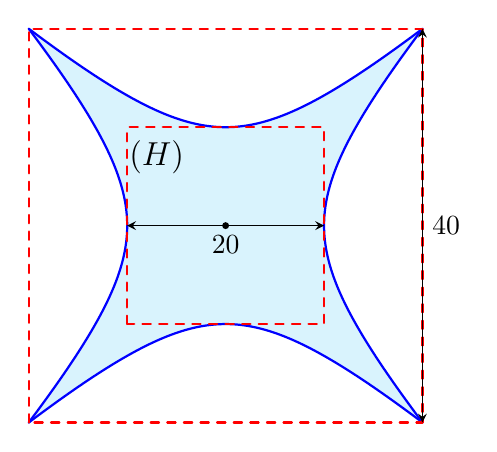
\begin{tikzpicture}[scale=0.125, >=stealth, line join=round, line cap=round]
			\fill[cyan!15]
			plot[domain=-20:20, samples=100] ({0.5*sqrt(400+3*\x*\x)}, \x) --
			plot[domain=20:-20, samples=100] (\x, {0.5*sqrt(400+3*\x*\x)}) --
			plot[domain=20:-20, samples=100] ({-0.5*sqrt(400+3*\x*\x)}, \x) --
			plot[domain=-20:20, samples=100] (\x, {-0.5*sqrt(400+3*\x*\x)}) -- cycle;
			\draw[blue, thick] plot[domain=-20:20, samples=100] ({0.5*sqrt(400+3*\x*\x)}, \x);
			\draw[blue, thick] plot[domain=-20:20, samples=100] ({-0.5*sqrt(400+3*\x*\x)}, \x);
			\draw[blue, thick] plot[domain=-20:20, samples=100] (\x, {0.5*sqrt(400+3*\x*\x)});
			\draw[blue, thick] plot[domain=-20:20, samples=100] (\x, {-0.5*sqrt(400+3*\x*\x)});
			\draw[red, dashed, thick] (-20,-20) rectangle (20,20);
			\draw[red, dashed, thick] (-10,-10) rectangle (10,10);
			\fill (0,0) circle (10pt);
			\draw[<->](-10,0)--(10,0) node[midway,below]{$20$};
			\draw[<->](20,-20)--(20,20) node[midway,right]{$40$};
			\node at (-7, 7) {\large $(H)$};
	\end{tikzpicture}}
	\par
	\shortans[0]{608}
	\loigiai{
		\begin{center}
			\begin{tikzpicture}[scale=0.15, >=stealth, line join=round, line cap=round]
				\fill[cyan!15]
				plot[domain=-20:20, samples=100] ({0.5*sqrt(400+3*\x*\x)}, \x) --
				plot[domain=20:-20, samples=100] (\x, {0.5*sqrt(400+3*\x*\x)}) --
				plot[domain=20:-20, samples=100] ({-0.5*sqrt(400+3*\x*\x)}, \x) --
				plot[domain=-20:20, samples=100] (\x, {-0.5*sqrt(400+3*\x*\x)}) -- cycle;
				\fill[pattern=north east lines, pattern color=orange]
				plot[domain=0:20, samples=50] ({0.5*sqrt(400+3*\x*\x)}, \x) -- (20,20) -- (0,0) -- (10,0) -- cycle;
				\draw[blue, thick] plot[domain=-20:20, samples=100] ({0.5*sqrt(400+3*\x*\x)}, \x);
				\draw[blue, thick] plot[domain=-20:20, samples=100] ({-0.5*sqrt(400+3*\x*\x)}, \x);
				\draw[blue, thick] plot[domain=-20:20, samples=100] (\x, {0.5*sqrt(400+3*\x*\x)});
				\draw[blue, thick] plot[domain=-20:20, samples=100] (\x, {-0.5*sqrt(400+3*\x*\x)});
				\draw[red, dashed, thick] (-20,-20) rectangle (20,20);
				\draw[red, dashed, thick] (-10,-10) rectangle (10,10);
				\draw[->, gray] (-25,0) -- (25,0) node[right, black] {$x$};
				\draw[->, gray] (0,-25) -- (0,25) node[above, black] {$y$};
				\fill (0,0) circle (10pt) node[below right] {$O$};
				\draw[dashed, gray!80!black] (-22,-22) -- (22,22) node[below right] {$y=x$};
				\fill (20,20) circle (10pt) node[above right] {$(20; 20)$};
				\fill (10,0) circle (10pt) node[below right] {$(10; 0)$};
				\node at (-7, 14) {\large $(H)$};
			\end{tikzpicture}
		\end{center}
		\textbf{Bước $1$: Gắn hệ trục tọa độ và tìm phương trình Hypebol}\\
		Chọn hệ trục tọa độ $Oxy$ sao cho gốc $O$ trùng với tâm của hai hình vuông, các cạnh hình vuông song song với các trục tọa độ.\\
		Khi đó, hình vuông nhỏ có các đỉnh là $(\pm 10; \pm 10)$, hình vuông lớn có các đỉnh là $(\pm 20; \pm 20)$.\\
		Nhánh hypebol bên phải có đỉnh nằm trên trục $Ox$ tại điểm $(10; 0)$ và đi qua góc của hình vuông lớn tại điểm $(20; 20)$.\\
		Giả sử phương trình hypebol giới hạn bên phải có dạng
		\[ \frac{x^2}{a^2} - \frac{y^2}{b^2} = 1 \]
		\begin{itemize}
			\item Đỉnh tại $(10; 0) \implies a = 10$.
			\item Đi qua $(20; 20) \implies \displaystyle \frac{20^2}{10^2} - \frac{20^2}{b^2} = 1 \implies 4 - \frac{400}{b^2} = 1 \implies b^2 = \frac{400}{3}$.
		\end{itemize}
		Phương trình nhánh hypebol bên phải là: $\displaystyle \frac{x^2}{100} - \frac{3y^2}{400} = 1 \implies x = \frac{1}{2}\sqrt{400 + 3y^2}$ (với $x > 0$).\\
		\textbf{Bước $2$: Phân tích tính đối xứng và tính diện tích}\\
		Do tính đối xứng, diện tích hình $(H)$ bằng $8$ lần diện tích phần $S_1$ nằm trong góc phần tư thứ nhất và bị giới hạn bởi
		\begin{itemize}
			\item Trục hoành $y=0$, đường phân giác $y=x$.
			\item Đường hypebol $x = \displaystyle \frac{1}{2}\sqrt{400 + 3y^2}$ (phần gạch trên hình vẽ).
		\end{itemize}
		Diện tích $S_1$ bằng cách tích phân theo biến $y$ từ $0$ đến $20$:
		\[ S_1 = \int\limits_{0}^{20} \left( \frac{1}{2}\sqrt{400 + 3y^2} - y \right) \mathrm{\,d}y = \dfrac{100}{\sqrt{3}}\ln\left(2+\sqrt{3}\right).\]
		Diện tích toàn bộ hình $(H)$ là
		\[ S = 8 S_1 = \dfrac{800}{\sqrt{3}}\ln\left(2+\sqrt{3}\right) \approx 608.\]
	}
\end{ex}

%%%============= EX_20 =============%%%
\begin{ex}%[2H5C1-7]%[TDMZZ12]%[Trương Tường]
	\immini[thm]{
		Trong không gian $Oxyz$ có đơn vị dài trên mỗi trục là mét, mặt đất là mặt phẳng $z+12=0$. Một vật $M$ được coi như một hạt chuyển động trên một quỹ đạo tròn ở ba thời điểm có ba vị trí là $A(2;1;10)$, $B(6;3;8)$, $C(8;5;6)$. Hãy tính theo đơn vị mét khoảng cách ngắn nhất tính từ vật đến mặt đất (không làm tròn các phép tính trung gian và kết quả cuối cùng được làm tròn đến hàng phần trăm).
	}{
		
		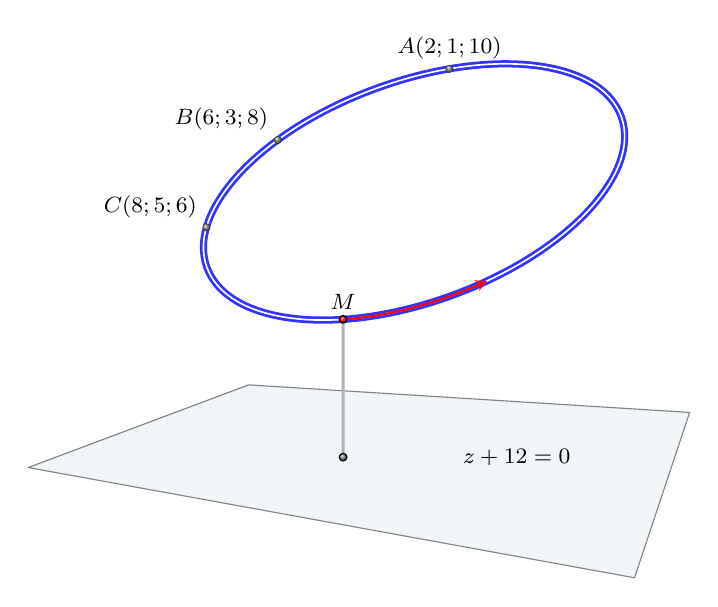
\begin{tikzpicture}[scale=0.7, >=stealth, line join=round, line cap=round, font=\footnotesize]
			\def\a{4} \def\b{2} \def\g{20}  
			\begin{scope}[rotate=\g]
				\foreach \x/\y in {70/A, 120/B, 160/C, -120/M}{
					\path ({\a*cos(\x)},{\b*sin(\x)}) coordinate (\y);	
				}
				\draw[line width=1pt, gray!10, double, blue!80] (0,0) ellipse ({\a} and {\b});
				\draw[->, red, thick] plot[domain=-120:-80] ({\a*cos(\x)},{\b*sin(\x)});
			\end{scope}
			\path (0,0) coordinate (I)
			\foreach \x/\y/\z in {-7/-5/1, -3/-3.5/2, 5/-4/3, 4/-7/4}{
				(\x,\y) coordinate (t\z)
			}
			(M)--++(-90:2.5) coordinate (H);
			\draw[fill=gray!70!cyan!10, draw=gray] (t1)--(t2)--(t3)--(t4)--cycle;
			\draw [line width=1pt, gray!60] (M)--(H);
			\foreach \x/\y/\z in {A/{2;1;10}/above, B/{6;3;8}/above left, C/{8;5;6}/above left}{
				\fill [ball color=gray] (\x) circle (2pt) node [\z] {$\x(\y)$};
			}
			\draw[ball color=red] (M) circle (2pt) node[above] {$M$};
			\draw[ball color=gray] (H) circle (2pt);
			\path (H)++(0:2) node[right] {$z+12=0$};
		\end{tikzpicture}
	}
	\par
	\shortans[0]{5,25}
	\loigiai{
		\begin{center}
			\begin{tikzpicture}[scale=1, >=stealth, line join=round, line cap=round, font=\footnotesize]
				\def\a{.6} \def\b{1.1} \def\g{30}
				\path (0,0) coordinate (P1)
				++(0:5) coordinate (P2)
				++(-135:2.5) coordinate (P3)
				++($(P1)-(P2)$) coordinate (P4)
				(P2)+(-2,4) coordinate (Q2)
				(P3)+(-2,4) coordinate (Q3)
				(intersection of P1--P2 and P3--Q3) coordinate (t)
				(barycentric cs:P3=.5,Q2=.6,P2=-.1) coordinate (I)
				(intersection cs: first line={(I)--++($(Q2)-(P2)$)}, second line={(P2)--(P3)}) coordinate (L)
				+($(Q2)-(P2)$) coordinate (L1)
				+($(P1)-(P2)$) coordinate (L2)
				;
				\foreach \t/\y in {10/A, 60/B, 130/C}{
					\path[rotate=\g] ($(I)+({0.6*cos(\t)},{1.1*sin(\t)})$) coordinate (\y);
				}
				\path [name path=k] (L)--(L1);
				\draw [name path=e, rotate=\g] (I) ellipse (.6 and 1.1);
				\path [name intersections={of=k and e, by={M',M}}];
				\path ($(L)!(M)!(L2)$) coordinate (H)
				($(H)!(I)!(L)$) coordinate (K)
				($(I)!(M)!(K)$) coordinate (N)
				;
				\pic [draw, "$P$", angle radius=0.5cm, angle eccentricity=.65] {angle=P3--P4--P1};
				%\pic [draw, "$Q$", angle radius=0.35cm, angle eccentricity=.55] {angle=P3--Q3--Q2};
				\pic [draw, angle radius=0.2cm] {angle=I--L--K};
				\pic [draw, angle radius=0.2cm] {angle=I--M--N};
				\foreach \x/\y/\z in {L/H/M, L/K/I, K/N/M, P2/L/M, H/L/P3}{
					\pic [draw, angle radius=0.1cm] {right angle=\x--\y--\z};
				}
				\draw [dash pattern=on 1pt off 2pt] (t)--(P2) (M)--(H)--(L) (I)--(K)--(H) (M)--(N);
				\draw (t)--(P1)--(P4)--(P3)--(P2) (P2)--(Q2)--(Q3)--(P3) (I)--(L);
				\foreach \x/\y in {I/90, L/-20, M/-30, H/-90, K/-90, N/190, A/70, B/90, C/120}{
					\draw [fill=black] (\x) circle (1pt) ++(\y:0.3) node {$\x$};
				}
				\draw (K)++(180:3) node[right] {$z+12=0$}
				(B)++(.5,.5)--++(0:1) node[right] {$(ABC)$}
				;
			\end{tikzpicture}
		\end{center}
		Gọi $I$ là tâm đường tròn $(C)$ ngoại tiếp tam giác $ABC$; $(\alpha)$, $(\beta)$ lần lượt là mặt phẳng trung trực của đoạn thẳng $AB$, $AC$. \\
		Khi đó, $I$ là giao điểm của ba mặt phẳng $(\alpha)$, $(\beta)$ và $(ABC)$. \\
		Gọi $D$, $E$ lần lượt là trung điểm của $AB$, $AC$. \\
		$\Rightarrow D(4;2;9)$ và $E(5;3;8)$. \\
		Ta có $\overrightarrow{AB}=(4;2;-2)$ là một vectơ pháp tuyến của $(\alpha)$, $\overrightarrow{AC}=(6;4;-4)$ là một vectơ pháp tuyến của $(\beta)$ và $\left[\overrightarrow{AB},\overrightarrow{AC}\right]=(0;4;4)$ là một vectơ pháp tuyến của $(ABC)$. \\
		Mặt phẳng $(ABC)$ có phương trình $0(x-2)+4(y-1)+4(z-10)=0 \Leftrightarrow y+z-11=0$. \\
		Mặt phẳng $(\alpha)$ có phương trình $4(x-4)+2(y-2)-2(z-9)=0 \Leftrightarrow 2x+y-z-1=0$. \\
		Mặt phẳng $(\beta)$ có phương trình $6(x-5)+4(y-3)-4(z-8)=0 \Leftrightarrow 3x+2y-2z-5=0$. \\
		Tọa độ điểm $I$ là nghiệm của hệ phương trình 
		\[\heva{&y+z-11=0 \\ &2x+y-z-1=0 \\ &3x+2y-2z-5=0} \Leftrightarrow \heva{&x=-3 \\ &y=9 \\ &z=2.}\]
		$\Rightarrow I(-3;9;2)$. \\
		Do đó bán kính đường tròn $(C)$ là $IA=\sqrt{(2+3)^2+(1-9)^2+(2-10)^2}=3\sqrt{17}$ (m). \\
		Gọi $M$ là điểm thuộc $(C)$ sao cho $M$ cách mặt phẳng $(P) \colon z+12=0$ một khoảng ngắn nhất. \\
		Gọi $H$ và $K$ lần lượt là hình chiếu vuông góc của $M$ và $I$ trên $(P)$; $N$ là hình chiếu vuông góc của $M$ trên $IK$. \\
		Khi đó $\mathrm{d}\left(M,(P)\right)=MH=NK=IK-IN$. \\
		Ta có $IK=\mathrm{d}(I,(P))=\dfrac{|2+12|}{\sqrt{0^2+0^2+1^2}}=14$ (m). \\
		Nhận xét rằng góc giữa hai mặt phẳng $(ABC)$ và $(P)$ là $\widehat{IMN}$. \\
		Mặt phẳng $(P)$ có vectơ pháp tuyến $\overrightarrow{n}=(0;0;1)$. \\
		Do đó $\cos\widehat{IMN}=\left|\cos\left(\overrightarrow{n},\overrightarrow{n'}\right)\right|=\dfrac{|0 \cdot 0+4 \cdot 0+4 \cdot 1|}{\sqrt{0^2+4^2+4^2} \cdot \sqrt{0^2+0^2+1^2}}=\dfrac{\sqrt{2}}{2}$. \\
		$\Rightarrow \widehat{IMN}=45^\circ$. \\
		$\Rightarrow \triangle IMN$ vuông cân tại $N$. \\
		$\Rightarrow IN=\dfrac{IM}{\sqrt{2}}=\dfrac{3\sqrt{17}}{\sqrt{2}}=\dfrac{3\sqrt{34}}{2}$ (m). \\
		Vậy $\mathrm{d}(M,(P))=IK-IN=14-\dfrac{3\sqrt{34}}{2} \approx 5{,}25$ (m). 
	}
\end{ex}

%%%============= EX_21 =============%%%
\begin{ex}%[1C2V3-2]%[TDMZZ12]%[Nguyễn Đức Tuấn Anh]
	\immini[thm]{
		Cho một mô hình $7$ trụ $A_1$, $A_2$, $A_3$, $A_4$, $A_5$, $A_6$, $S$ có đỉnh $S$ nối với $6$ trụ còn lại với các thử thách trên đường đi giữa $S$ và các trụ $A_i$ $(i \in \{1; 2; 3; 4; 5; 6\})$ là $30+i$, các đỉnh còn lại tạo với nhau thành một đa giác $A_1 A_2 A_3 A_4 A_5 A_6$ với thử thách nối hai đỉnh $A_i$, $A_j$ $(i, j \in \{1; 2; 3; 4; 5; 6\})$ là $5+2i+2j$. Một đường đi tinh gọn là một đường đi mà người chơi sẽ xuất phát từ một trụ nào đó, đi qua tất cả các trụ (mỗi khi đi qua một trụ thì trụ đó bị phá hủy và không thể đi lại được nữa), rồi cuối cùng người chơi phải trở về trụ ban đầu. Hãy xác định tổng thử thách nhỏ nhất có thể của một đường đi tinh gọn?}{
		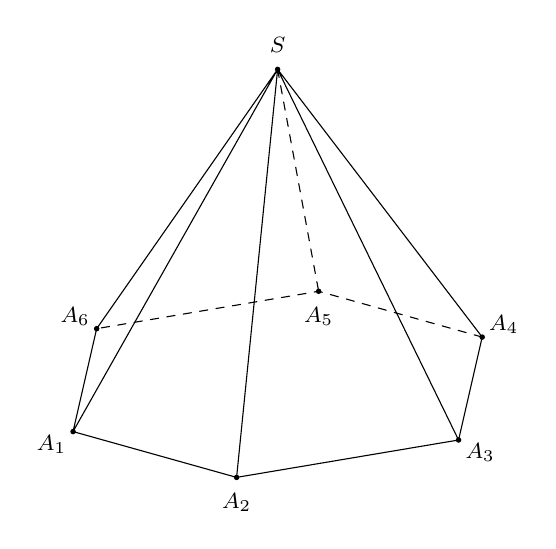
\begin{tikzpicture}[line cap=round, line join=round, >=stealth, font=\footnotesize]
			\path (0,4) coordinate (S)
			(210:3 and 1.2) coordinate (A_1)
			(260:3 and 1.2) coordinate (A_2)
			(320:3 and 1.1) coordinate (A_3)
			(30:3 and 1.2)  coordinate (A_4)
			(80:3 and 1.2)  coordinate (A_5)
			(140:3 and 1.1) coordinate (A_6);
			\draw (A_1) -- (A_2) -- (A_3) -- (A_4)
			(S) -- (A_1) (S) -- (A_2) (S) -- (A_3) (S) -- (A_4) (S) -- (A_6)-- (A_1);
			\draw[dashed] (A_4) -- (A_5) -- (A_6)  
			(S) -- (A_5);
			\foreach \t/\g in {S/90, A_1/210, A_2/-90, A_3/-30, A_4/30, A_5/-90, A_6/150}{
				\fill (\t) circle (1pt) node[shift={(\g:9pt)}]{$\t$};
			}
		\end{tikzpicture}
	}
	\par
	\shortans[0]{158}
	\loigiai{
		\begin{center}
			\begin{tikzpicture}[line cap=round, line join=round, >=stealth, font=\footnotesize,mid arrow/.style={
					postaction={
						decorate,
						decoration={
							markings,
							mark=at position 0.5 with {\arrow{>}}
						}
					}
				}]
				\path (0,4) coordinate (S)
				(210:3 and 1.2) coordinate (A_1)
				(260:3 and 1.2) coordinate (A_2)
				(320:3 and 1.1) coordinate (A_3)
				(30:3 and 1.2)  coordinate (A_4)
				(80:3 and 1.2)  coordinate (A_5)
				(140:3 and 1.1) coordinate (A_6);
				\foreach \x/\y in {1/2,2/3,3/4}{\draw[mid arrow] (A_\x)--(A_\y);}
				\draw[mid arrow] (S)--(A_1);
				\draw[mid arrow] (A_6)--(S);
				\draw[dashed,mid arrow] (A_4)--(A_5);
				\draw[dashed,mid arrow] (A_5)--(A_6);
				\draw
				(S) -- (A_1) (S) -- (A_2) (S) -- (A_3) (S) -- (A_4) (S) -- (A_6)--(A_1);
				\draw[dashed]
				(S) -- (A_5);
				\foreach \t/\g in {S/90, A_1/210, A_2/-90, A_3/-30, A_4/30, A_5/-90, A_6/150}{
					\fill (\t) circle (1pt) node[shift={(\g:9pt)}]{$\t$};
				}
			\end{tikzpicture}
		\end{center}
		Xét một đường đi tinh gọn bất kì, đường đi này đi qua toàn bộ $7$ đỉnh nên sẽ gồm $5$ cạnh liên kết các đỉnh ở đáy với nhau và $2$ cạnh bên đi qua đỉnh $S$.\\
		Ta có thể xem đường đi ở đáy được tạo ra bằng cách lấy một chu trình đi qua $6$ đỉnh ở đáy, sau đó bỏ đi $1$ cạnh $A_iA_j$.\\
		Khi đó, để hoàn thành đường đi tinh gọn qua tất cả các trụ, ta nối thêm $2$ cạnh bên là $SA_i$ và $SA_j$.\\
		Tổng trọng số của $6$ cạnh tạo thành chu trình đáy bất kì là
		\[ 6 \cdot 5 + 2 \cdot \big[2(1+2+3+4+5+6)\big] = 30 + 2 \cdot 42 = 114. \]
		Suy ra, tổng đường đi tinh gọn $S \to A_i \to \dots \to A_j \to S$ là
		\begin{align*}
			T &= 114 - A_iA_j + SA_i + SA_j \\
			&= 114 - \big[5 + 2(i+j)\big] + 30 + i + 30 + j \\
			&= 169 - (i+j).
		\end{align*}
		Để tổng thử thách $T$ là nhỏ nhất thì $(i+j)$ phải đạt giá trị lớn nhất.\\
		Vì $i$, $j \in \{1; 2; 3; 4; 5; 6\}$ và phân biệt nên ta có $i+j \le 5 + 6 = 11$.\\
		Do đó
		\[ T \ge 169 - 11 = 158. \]
		Dấu bằng xảy ra khi và chỉ khi $(i, j) = (5, 6)$ hoặc $(i, j) = (6, 5)$.\\
		Một đường đi thỏa mãn cho tổng thử thách nhỏ nhất là $S \to A_5 \to A_4 \to A_3 \to A_2 \to A_1 \to A_6 \to S$.\\
		Vậy tổng thử thách nhỏ nhất có thể của một đường đi tinh gọn là $158$.
	}
\end{ex}

%%%============= EX_22 =============%%%
\begin{ex}%[2D6C2-3]%[TDMZZ12]%[Tên Tác Giả]
	Cho hai hộp, ban đầu hộp I đựng $10$ viên bi đỏ và $5$ viên bi xanh, những viên bi này có cùng kích thước và cùng khối lượng, còn hộp II chưa đựng gì. Tiến hành lấy ngẫu nhiên $7$ viên bi từ hộp I sang hộp II, gọi $A$ là biến cố hộp II lúc này có $5$ bi đỏ. Sau đó, tiến hành lấy ngẫu nhiên từ hộp II ra $4$ viên bi, gọi $B$ là biến cố lấy được đúng ba viên bi đỏ từ hộp II. Hãy tính xác suất $\mathrm{P}(A\mid B)$ (\textit{không làm tròn các phép tính trung gian và kết quả cuối cùng được làm tròn đến hàng phần trăm})?
	\par
	\shortans[0]{0,51}
	\loigiai{
		Số viên bi ban đầu ở hộp I là $15$ viên ($10$ đỏ, $5$ xanh).\\
		Ta có $\mathrm{P}(A) = \dfrac{\mathrm{C}_{10}^5 \cdot \mathrm{C}_5^2}{\mathrm{C}_{15}^7}=\dfrac{56}{143}$.\\
		Để tính $\mathrm{P}(B)$, ta coi việc lấy $4$ viên bi trong đó có đúng $3$ viên bi đỏ từ hộp II là lấy được $4$ viên bi trong đó có đúng $3$ viên bi đỏ từ hộp I (ban đầu).\\
		Khi đó $\mathrm{P}(B) = \dfrac{\mathrm{C}_{10}^3 \cdot \mathrm{C}_5^1}{\mathrm{C}_{15}^4}=\dfrac{40}{91}$.\\
		Mặt khác $\mathrm{P}\left(B\mid A\right)=\dfrac{\mathrm{C}_{5}^3 \cdot \mathrm{C}_2^1}{\mathrm{C}_{7}^4}=\dfrac{4}{7}$.\\
		Xác suất cần tìm theo công thức Bayes là
		\[\mathrm{P}(A\mid B) = \frac{\mathrm{P}(A)\cdot\mathrm{P}\left(B\mid A\right) }{\mathrm{P}(B)} =\dfrac{\dfrac{56}{143}\cdot \dfrac{4}{7}}{\dfrac{40}{91}}=\dfrac{28}{55}\approx 0{,}51.\]
	}
\end{ex}
